\documentclass[10pt,twocolumn,letterpaper]{article}

\usepackage[letterpaper,top=0.85in,bottom=0.9in,left=0.65in,right=0.65in,columnsep=0.28in]{geometry}
\usepackage{amsmath}
\usepackage[T1]{fontenc}
\usepackage{stix2}                 % body and math font (as in the Milestone 1 and 2 reports)
\usepackage[scaled=0.92]{helvet}   % sans font for title, headings and captions
\usepackage{microtype}
\usepackage{graphicx}
\usepackage{booktabs}
\usepackage{tabularx}
\usepackage{caption}
\usepackage{enumitem}
\usepackage{xcolor}
\usepackage{titlesec}
\usepackage{fancyhdr}
\usepackage{lastpage}
\usepackage[colorlinks=true,linkcolor=blue!50!black,citecolor=blue!50!black,urlcolor=blue!50!black]{hyperref}

\definecolor{titleblue}{RGB}{24,64,120}
\graphicspath{{figures/}}
\setlist{itemsep=2pt,topsep=4pt,leftmargin=*}
\captionsetup{font=small,labelfont={bf,sf},labelsep=period}
\newcommand{\code}[1]{\texttt{\detokenize{#1}}}

% headings: sans, numbered "1. Abstract", "4.1. ..."
\titleformat{\section}{\sffamily\bfseries\large\color{titleblue}}{\thesection.}{0.5em}{}
\titleformat{\subsection}{\sffamily\bfseries\normalsize}{\thesubsection.}{0.5em}{}
\titleformat{\paragraph}[runin]{\sffamily\bfseries\small}{}{0pt}{}
\titlespacing*{\section}{0pt}{12pt}{6pt}
\titlespacing*{\subsection}{0pt}{9pt}{4pt}
\titlespacing*{\paragraph}{0pt}{6pt}{0.5em}

% let full-width figures share pages with text
\renewcommand{\topfraction}{0.9}
\renewcommand{\dbltopfraction}{0.9}
\renewcommand{\textfraction}{0.1}
\renewcommand{\floatpagefraction}{0.8}
\renewcommand{\dblfloatpagefraction}{0.8}
\setcounter{topnumber}{2}
\setcounter{dbltopnumber}{1}   % at most one full-width float per page, so text always flows below it

\newcommand{\reporttitle}{Where Help Is Far Away: Four Types of Under-Served Wildfire Country}
\newcommand{\shorttitle}{Where Help Is Far Away: Types of Under-Served Wildfire Areas}

\pagestyle{fancy}
\fancyhf{}
\renewcommand{\headrulewidth}{0pt}
\fancyhead[R]{\footnotesize\itshape\shorttitle}
\fancyfoot[L]{\footnotesize\sffamily\textbf{\thepage}\quad CSEN 281}
\fancyfoot[R]{\footnotesize\sffamily Santa Clara University\quad\textbf{November, 2026}\quad Milestone 3 Report}
\fancypagestyle{first}{%
  \fancyhf{}
  \fancyfoot[L]{\footnotesize\sffamily CSEN 281}
  \fancyfoot[R]{\footnotesize\sffamily Santa Clara University\quad\textbf{November, 2026}\quad Milestone 3 Report\quad\textbf{1--\pageref{LastPage}}}%
}

\begin{document}
\twocolumn[{%
\begin{flushleft}
{\sffamily\bfseries\small CSEN 281 - Capstone Milestone 3 Report}\par\vspace{8pt}
{\sffamily\bfseries\LARGE\color{titleblue}\reporttitle\par}\vspace{8pt}
{\sffamily\bfseries\normalsize Quan Do\textsuperscript{a} and Nandingoo Erdenebat\textsuperscript{b}\par}\vspace{6pt}
{\footnotesize\itshape \textsuperscript{a}CSEN - qldo@scu.edu\\
\textsuperscript{b}CSEN -nerdenebat@scu.edu\par}
\end{flushleft}
\vspace{14pt}
}]
\thispagestyle{first}

%=====================================================================
\section{Abstract}
%=====================================================================
Milestones~1 and~2 showed that fires far from a fire station are much more likely to become large. This milestone asks what kinds of places those are. We divide the lower 48 states into 25~km grid cells and describe each cell by how its 1992--2018 fires behave. Inputs are fire rate, cyclically encoded season and discovery hour, weekend share, station access and land-owner shares; cause, size, reporting agency and region are held out. We then cluster the 2{,}016 \emph{under-served} cells, where the median fire is 10~km or more from a station. These cells hold 11.9\% of fires but 38.1\% of the acres burned. The internal indices disagree on the number of clusters, so $k$ is chosen by a bootstrap-stability rule fixed in advance. That rule gives $k=4$: 92\% of resampled pairs agree with adjusted Rand index (ARI) above 0.8. The four types are remote federal wildlands, federal forests with partial coverage, private-land spring fires and tribal lands. They separate held-out lightning share ($\eta^2=0.46$), reporting agency ($\eta^2=0.60$) and region (Cram\'er's $V=0.43$), and 84.7\% of cells keep their type when re-assigned from 2019--2024 fires alone ($\kappa=0.78$). A complementary association-rule pass, with thresholds derived from a precision target and a Bonferroni bound, finds 121 rules, 98\% of which keep lift above 1 on 2019--2024. The two analyses agree on where the largest fires are: remote federal land, private parcels far from stations, and \emph{sparse} cells with almost no fire history, which hold 26 of the 100 largest fires.

%=====================================================================
\section{Problem and Approach}
%=====================================================================
\begin{description}[leftmargin=0pt]
\item[RQ2 (unsupervised, clustering).] \emph{Among areas that have fires but no fire station nearby, what distinct types exist, and what kind of help would each type need?}
\end{description}
A single fire is too noisy to describe a place, so we cluster \emph{places}: each $\approx$25$\times$25~km grid cell becomes one point, described by averages over its fires. Two choices set this version apart from the preliminary clustering in Milestone~1. First, \textbf{fire-size features are held out}. In Milestone~1 they were inputs, which made the clusters partly circular with the RQ1 target. Second, \textbf{the typology is built on 1992--2018 only}, so 2019--2024 can test whether the types persist. A fire-level association-rule pipeline gives a second, more fine-grained view of the same question.

All results come from one notebook, \code{unsupervised_learning/unsupervised_learning.ipynb}.

%=====================================================================
\section{Data and Feature Space}
%=====================================================================
We use the FPA-FOD 7th edition \cite{short2026} joined to the 52{,}057 HIFLD fire and EMS stations \cite{hifld}, the cached table from Milestone~2. Two administrative columns are added for held-out checks: \code{NWCG_REPORTING_AGENCY} and \code{COMPLEX_NAME}. We keep the 2{,}603{,}776 lower-48 fires that are not on stacked office coordinates: 2{,}120{,}539 in 1992--2018 and 483{,}237 in 2019--2024.

\paragraph{Fire-level encodings.} Day of year and discovery hour are put on the unit circle so that 31~December and 1~January, or 23:00 and 00:00, are neighbours:
\begin{align}
(s_d, c_d) &= \big(\sin\tfrac{2\pi\,\text{doy}}{365.25},\ \cos\tfrac{2\pi\,\text{doy}}{365.25}\big),\\
(s_h, c_h) &= \big(\sin\tfrac{2\pi(h+0.5)}{24},\ \cos\tfrac{2\pi(h+0.5)}{24}\big).
\end{align}
The 17 raw land-owner codes, a high-cardinality categorical with two codes differing only in case, are collapsed into five groups: federal, private, state/local, tribal (including BIA trust land) and missing. The missing group is 40\% of fires and is a reporting artefact (Milestone~1), so it is the left-out reference share.

\paragraph{Cell features.} A cell's circular means $(\bar s, \bar c)$ carry both the timing (the angle of the mean vector) and how concentrated it is (its length). Table~\ref{tab:features} lists the 12 inputs. A cell is \emph{described} if it has 30 or more fires and \emph{under-served} if its median fire is 10~km or more from the nearest station. Of 12{,}902 occupied cells, 8{,}025 are described and 2{,}016 are under-served. The 28 cells with no recorded discovery time get the median cell's diurnal pair. All inputs are then standardised.

\begin{table}[!htb]
\centering\small
\caption{Clustering inputs (12) and held-out variables. All are cell averages over 1992--2018 fires.}
\label{tab:features}
\begin{tabularx}{\columnwidth}{@{}lX@{}}
\toprule
Group & Features \\
\midrule
Activity & \code{log_fire_rate} = $\log(1+\text{fires/yr})$ \\
Timing & \code{season_sin}, \code{season_cos}, \code{hour_sin}, \code{hour_cos}, \code{weekend_share} \\
Access & \code{log_median_dist} (km to nearest station), \code{log1p_stations_25km} \\
Owner & federal, private, state/local and tribal shares \\
\midrule
\emph{Held out} & lightning share, large-fire share, median $\log_{10}$ size, missing discovery time, missing cause, state/local-reported share, complex share, region \\
\bottomrule
\end{tabularx}
\end{table}

\paragraph{Is there structure?} The Hopkins statistic is 0.83 (0.82--0.84 over 10 draws), far above the 0.5 of uniform noise. PCA needs 9 of 12 components for 90\% of the variance. The strongest input correlation is distance vs station count ($|r|=0.81$); no other pair exceeds 0.62.

%=====================================================================
\section{Methods}
%=====================================================================
\subsection{Choosing $k$}
For $k=2,\dots,10$ we report the elbow, silhouette, Davies--Bouldin (DB), Calinski--Harabasz (CH) and the gap statistic \cite{tibshirani2001}. Internal indices reward compact, separated groups but say nothing about whether the same groups return when the data change. We therefore fix a stability rule before looking at any cluster profile \cite{benhur2002}. We draw $B=50$ pairs of bootstrap resamples, fit K-Means (\code{n_init}=10) to each, label every cell with both fits and compute
\begin{equation}
S_k = \big\{\text{ARI}(f^{(1)}_b(X), f^{(2)}_b(X))\big\}_{b=1}^{B},
\end{equation}
and choose
\begin{equation}
k^\ast = \max\{k : \tfrac{1}{B}\textstyle\sum_b \mathbb{1}[S_{k,b} > 0.8] \geq 0.9\},
\end{equation}
the most detailed partition that is reproducible in at least 90\% of resamples.

\subsection{Algorithms}
\textbf{K-Means} (50 restarts) is the main model. Three other families test whether a different inductive bias finds different structure: a \textbf{Gaussian mixture} (full and diagonal covariance, BIC over $k$); \textbf{Ward agglomerative} clustering; and \textbf{HDBSCAN} \cite{campello2013}, swept over minimum cluster sizes of 10--100 in the full space and in the first three principal components. K-Means is also refitted on the 9 principal components that cover 90\% of the variance, to check that correlated inputs are not double-counted.

\subsection{Validation}
\textbf{Held-out variables.} $\eta^2$ (share of between-cell variance explained by type) for numeric variables, Cram\'er's $V$ for region, and the share of the 100 largest 1992--2018 fires and of all \emph{complex} fires falling in each type. \textbf{Temporal.} For every under-served cell with 10+ fires in 2019--2024 we recompute the inputs from those fires alone. We standardise them with the 1992--2018 scaler, assign each cell to the nearest 1992--2018 centre and measure agreement with Cohen's $\kappa$. \textbf{Ablation.} We drop one feature group at a time and compare the refit partition with the full one by ARI.

\subsection{Association rules}
Each fire is a transaction with one item per attribute: region, season, owner group, distance band ($<$5, 5--10, 10--20, 20+~km), cause class, discovery period (day, night, unknown), weekend, and \emph{cell class}. The cell class is one of the four types, a \emph{served} cell, or a \emph{sparse} cell with fewer than 30 fires. The consequent is always \code{LARGE} ($\geq$100 acres). Because each transaction has exactly one item per attribute, enumerating all attribute combinations of length 1--3 with a group-by returns exactly the frequent itemsets Apriori \cite{agrawal1994} would find, with exact counts. Rules are mined on 1992--2018 and scored once on 2019--2024. The three thresholds are derived, not picked:

\paragraph{Support.} With base rate $p_0$, we require the 95\% interval of a rule's confidence to be no wider than $\pm 25\%$ of $p_0$ even at lift 1:
\begin{equation}
1.96\sqrt{\frac{p_0(1-p_0)}{n}} \le 0.25\,p_0 \;\Rightarrow\; n \ge \frac{1.96^2(1-p_0)}{0.25^2\,p_0}.
\end{equation}
With $p_0=2.857\%$ this gives $n_{\min}=2{,}091$ fires, a minimum support of 0.099\%.

\paragraph{Confidence and lift.} With $m$ candidate rules, a rule is kept only if the one-sided Bonferroni-corrected Wilson lower bound $\ell$ of its confidence satisfies $\ell/p_0 \ge 2$ ($z = \Phi^{-1}(1-0.05/m)$). We are then 95\% confident, family-wise, that matching fires are at least twice as likely as average to become large.

\paragraph{Non-redundancy.} A longer rule must have $\ell$ above the point confidence of every one of its sub-rules (minimum improvement \cite{bayardo2000}).

%=====================================================================
\section{Results}
%=====================================================================
% full-width figures can only appear at the top of a later page, so each is defined about a page before it is discussed
\begin{figure*}[t]
\centering
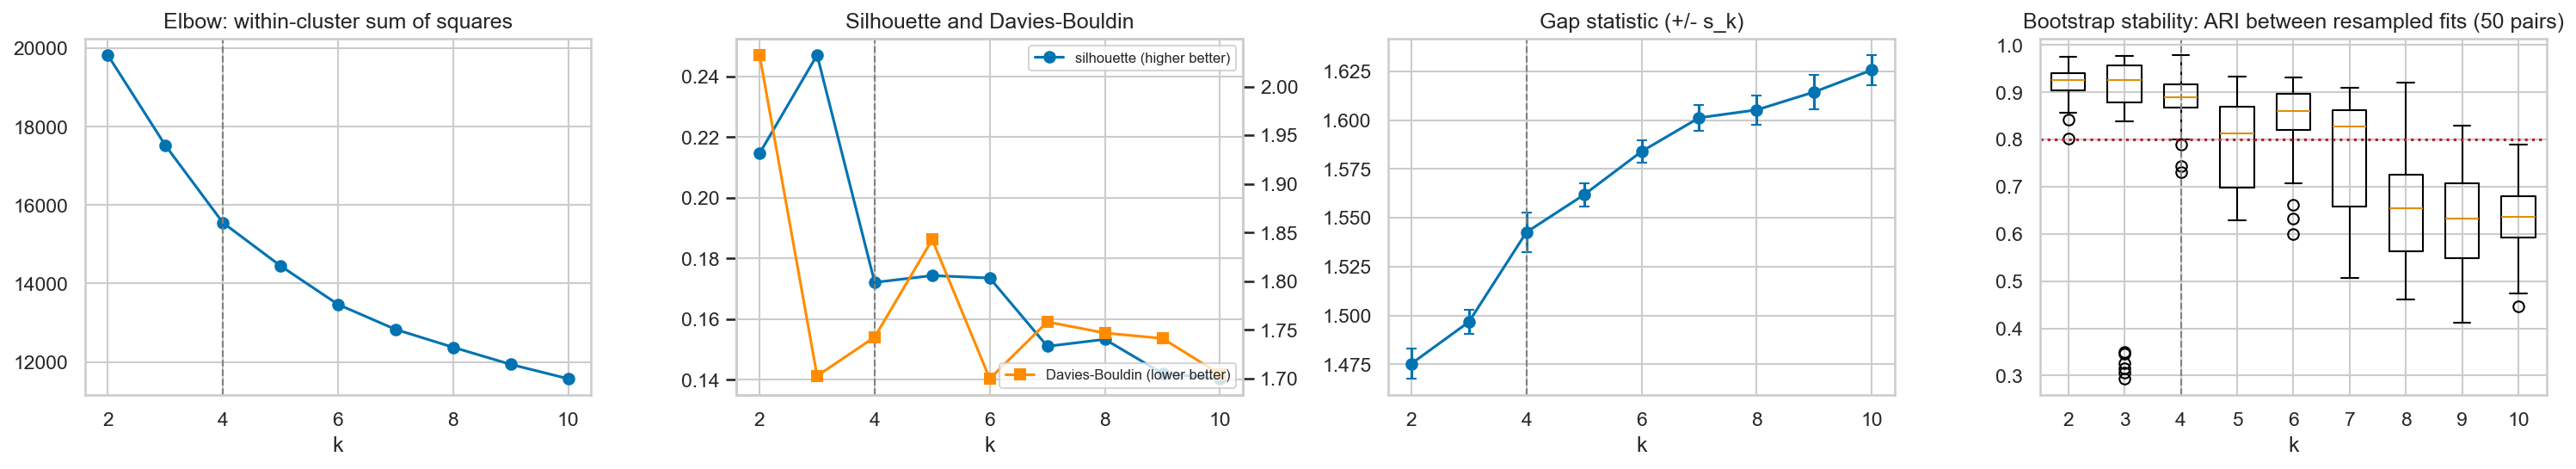
\includegraphics[width=\textwidth]{model_selection.png}
\caption{Choosing $k$ on the 2{,}016 under-served cells. From left: elbow; silhouette (blue) and Davies--Bouldin (orange); gap statistic; and the bootstrap stability distribution, the ARI between two K-Means fits on independent resamples (50 pairs per $k$). The dashed line marks the chosen $k=4$.}
\label{fig:selection}
\end{figure*}

\subsection{Number of clusters}
The internal indices disagree (Table~\ref{tab:k}, Figure~\ref{fig:selection}). Silhouette is best at $k=3$, CH at $k=2$, and DB is almost flat (1.70 at $k=3$, 6 and 10). The elbow has no clear bend, and the gap statistic rises until $k=7$. This pattern is typical of overlapping groups. Stability decides: $k=3$ has the best silhouette but splits two ways, and 12\% of its bootstrap pairs disagree badly (ARI about 0.3). $k=4$ is the largest $k$ meeting the rule, with 92\% of pairs above 0.8 and a median ARI of 0.89. Beyond it, agreement collapses (52\% at $k=5$, 10\% at $k=8$). The price is a lower silhouette, 0.17, so the four types are best read as regimes with clear cores and fuzzy borders.

\begin{table}[!htb]
\centering\footnotesize
\setlength{\tabcolsep}{4pt}
\caption{K-Means model selection. Stab.\ = mean bootstrap ARI; ``$>$0.8'' = share of pairs with ARI above 0.8 (rule: $\geq$0.9). Best value per column in bold.}
\label{tab:k}
\begin{tabular}{@{}ccccccc@{}}
\toprule
$k$ & Silh. & DB & CH & Gap & Stab. & $>$0.8 \\
\midrule
2 & 0.215 & 2.03 & \textbf{443} & 1.48 & \textbf{0.92} & \textbf{1.00} \\
3 & \textbf{0.247} & \textbf{1.70} & 383 & 1.50 & 0.85 & 0.88 \\
\textbf{4} & 0.172 & 1.74 & 373 & 1.54 & 0.88 & \textbf{0.92} \\
5 & 0.174 & 1.84 & 339 & 1.56 & 0.79 & 0.52 \\
6 & 0.174 & \textbf{1.70} & 320 & 1.58 & 0.85 & 0.82 \\
7 & 0.151 & 1.76 & 297 & 1.60 & 0.76 & 0.56 \\
8 & 0.153 & 1.75 & 274 & 1.61 & 0.66 & 0.10 \\
\bottomrule
\end{tabular}
\end{table}

\subsection{Algorithm families}
K-Means on the 9 principal components reproduces the partition almost exactly (ARI 0.975), so correlated inputs are not distorting it. Ward clustering agrees moderately (0.56): the cores match and border cells move. The other two families do not find better structure. The Gaussian mixture's BIC keeps falling up to $k=10$ for both covariance types, and at $k=4$ it agrees poorly with K-Means (ARI 0.19). The owner shares pile up at exactly 0 and 1, and the mixture spends components on those point masses. HDBSCAN labels 37--100\% of cells as noise in the full space and finds only two clusters in three principal components. The cells form a continuum with dense cores rather than density-separated islands, which is why a partitioning method with a stability check fits the data better.

\begin{figure*}[t]
\centering
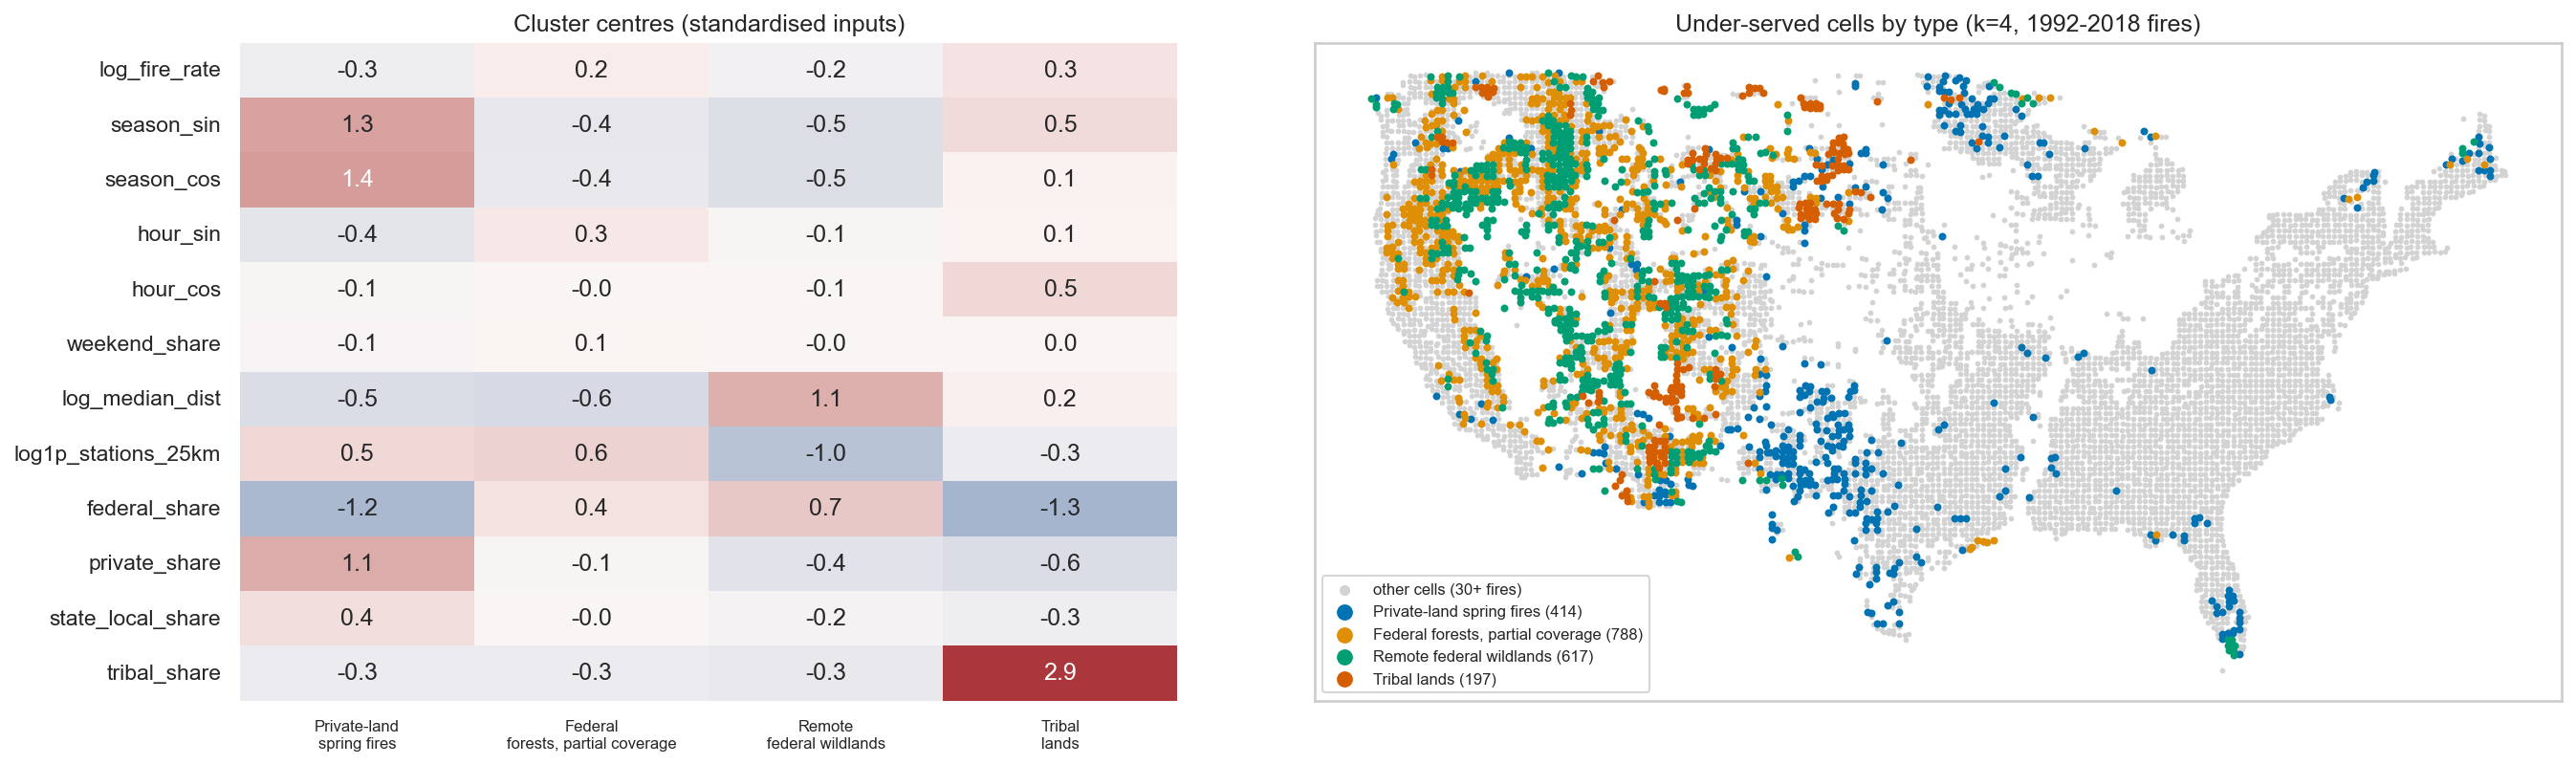
\includegraphics[width=\textwidth]{cluster_profile_map.png}
\caption{The four types ($k=4$). Left: cluster centres in standardised units. Right: under-served cells coloured by type. Grey cells have 30+ fires but are not under-served. Coordinates were never an input.}
\label{fig:types}
\end{figure*}

\subsection{The four types}
Table~\ref{tab:types} and Figure~\ref{fig:types} describe the types. They are separated by \emph{who owns the land}, \emph{when fires happen} and \emph{how far help is}; weekend share and discovery hour barely differ. Although coordinates were never an input, each type forms coherent regions on the map. Remote federal wildlands fill the Great Basin, central Idaho, Wyoming and the Arizona--New Mexico border. Federal forests with partial coverage line the Cascades, the Sierra Nevada and the Rockies. Tribal lands match the large reservations of the Southwest and northern Plains. Private-land spring fires sit in Texas and Oklahoma, Florida and northern Minnesota.

\begin{table}[!htb]
\centering\footnotesize
\setlength{\tabcolsep}{3pt}
\caption{Profiles of the four types (means over cells). Peak = day of year of the seasonal mean vector; conc.\ = its length (1 = all fires on one day). Stations = median count within 25~km.}
\label{tab:types}
\begin{tabular}{@{}lcccc@{}}
\toprule
 & Private & Federal & Remote & Tribal \\
 & spring & partial & federal & lands \\
\midrule
Cells & 414 & 788 & 617 & 197 \\
Fires per cell & 96 & 140 & 102 & 196 \\
Median km to station & 14.9 & 14.5 & \textbf{30.4} & 20.4 \\
Stations within 25 km & 2.5 & 2.7 & \textbf{0.2} & 1.0 \\
Federal share & 0.09 & 0.69 & \textbf{0.83} & 0.05 \\
Private share & \textbf{0.44} & 0.17 & 0.10 & 0.07 \\
Tribal share & 0.02 & 0.02 & 0.01 & \textbf{0.83} \\
Seasonal peak (day) & 150 & 210 & 211 & 192 \\
Seasonal conc. & 0.32 & 0.75 & 0.80 & 0.56 \\
Silhouette & 0.09 & 0.17 & 0.20 & 0.27 \\
\bottomrule
\end{tabular}
\end{table}

\begin{figure*}[t]
\centering
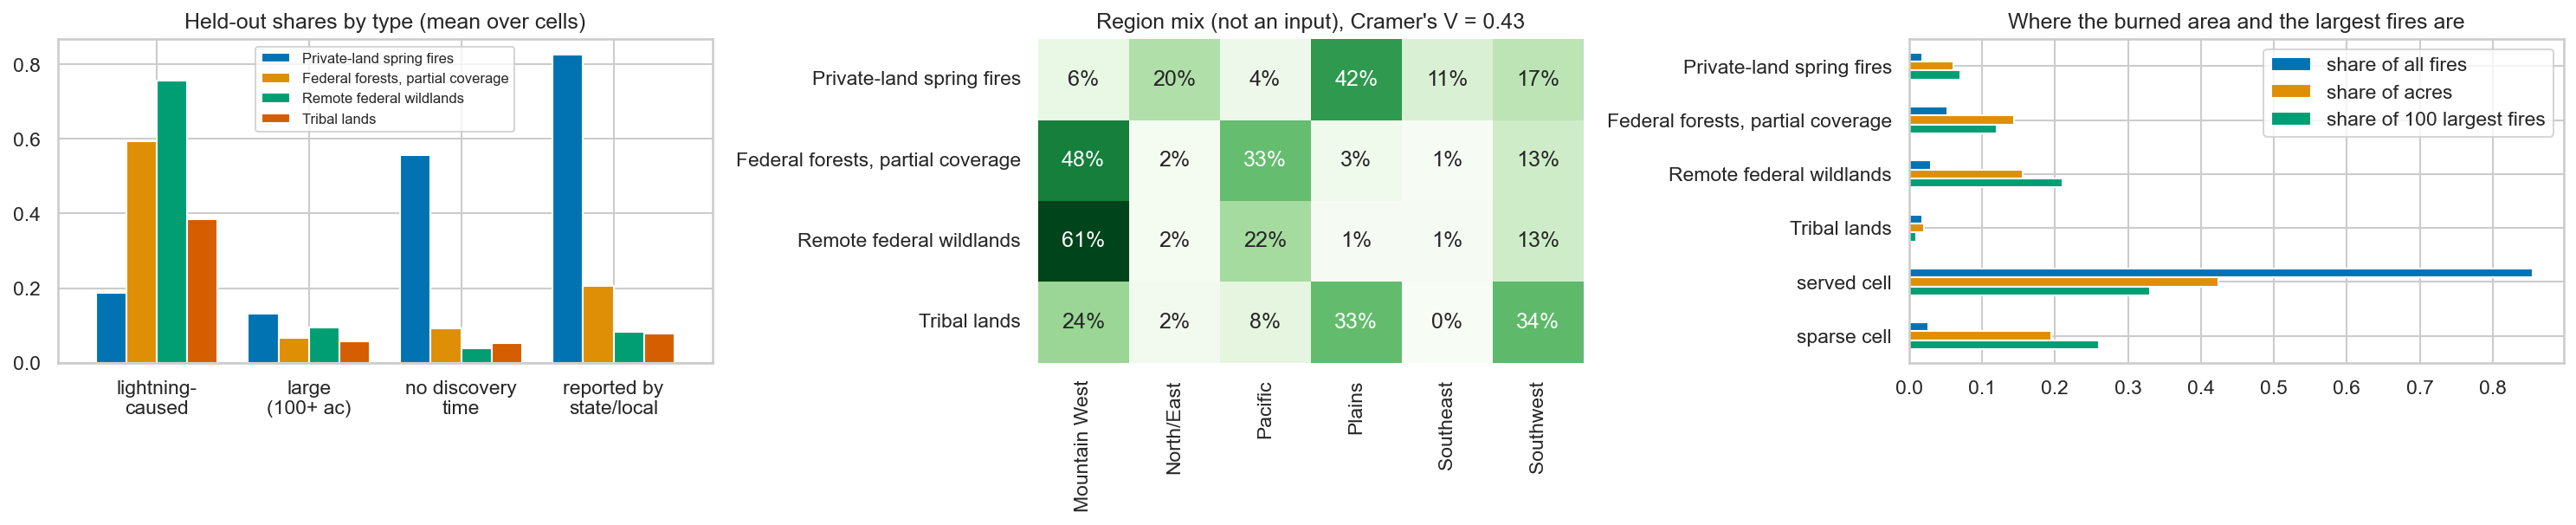
\includegraphics[width=\textwidth]{heldout_validation.png}
\caption{Held-out checks, 1992--2018. Left: cell-mean shares of held-out variables by type. Middle: region mix of each type. Right: share of all fires, of acres burned and of the 100 largest fires in each cell class. \emph{Served} = 30+ fires and median fire within 10~km; \emph{sparse} = fewer than 30 fires.}
\label{fig:heldout}
\end{figure*}

\subsection{Held-out validation}
\paragraph{Cause.} The types separate cause strongly even though it was never an input ($\eta^2=0.46$, Table~\ref{tab:heldout}): 76\% of fires in remote federal wildlands are lightning-caused, against 19\% in private-land spring fires.

\paragraph{Administrative reporting patterns} are the strongest signal of all (Figure~\ref{fig:heldout}). 83\% of private-land fires are reported by state or local agencies and 56\% have no discovery time, against 4--9\% for the other types ($\eta^2$ = 0.60 and 0.53). Without using any agency label, the clustering has recovered the federal/non-federal reporting divide that Milestone~1 found in the missing values.

\paragraph{Region} also lines up with the types (Cram\'er's $V=0.43$): remote wildlands are 61\% Mountain West, and private-land spring fires 42\% Plains.

\paragraph{Fire complexes and anomalies.} Fire size differs less ($\eta^2=0.07$ for the large-fire share). But the two federal types, with only 8.2\% of fires, hold 49\% of all complex fires, 30\% of the acres and 33 of the 100 largest fires. \emph{Sparse} cells, too thinly populated to cluster, hold 2.7\% of fires but 19.5\% of the acres and 26 of the 100 largest fires.

\begin{table}[!htb]
\centering\footnotesize
\setlength{\tabcolsep}{3.5pt}
\caption{Held-out variables by type (cell means) and the share of cell-level variance explained by type ($\eta^2$).}
\label{tab:heldout}
\begin{tabular}{@{}lccccc@{}}
\toprule
 & Priv. & Fed. & Rem. & Trib. & $\eta^2$ \\
\midrule
Lightning-caused & 0.19 & 0.60 & \textbf{0.76} & 0.39 & 0.46 \\
Large (100+ ac) & \textbf{0.13} & 0.07 & 0.09 & 0.06 & 0.07 \\
No discovery time & \textbf{0.56} & 0.09 & 0.04 & 0.05 & 0.53 \\
State/local report & \textbf{0.83} & 0.21 & 0.08 & 0.08 & 0.60 \\
Cause missing & 0.08 & 0.04 & 0.02 & 0.01 & 0.08 \\
\midrule
\multicolumn{5}{@{}l}{Region (Cram\'er's $V$)} & 0.43 \\
\bottomrule
\end{tabular}
\end{table}

\subsection{Temporal validation}
The types persist (Figure~\ref{fig:temporal}): 84.7\% of the 1{,}288 cells with 10+ fires in 2019--2024 keep their type ($\kappa=0.78$). Private-land (92\%) and tribal (91\%) cells are the most stable. Federal forests lose 15\% to the private type, partly because owner coding changed in 2020--21. The held-out large-fire rate still differs by type, but the order changed. Remote federal wildlands rose from 6.7\% to 9.2\% (95\% CI 8.6--9.8\%) and are now the highest, while private-land spring fires fell from 9.9\% to 8.6\%.

\begin{figure}[!htb]
\centering
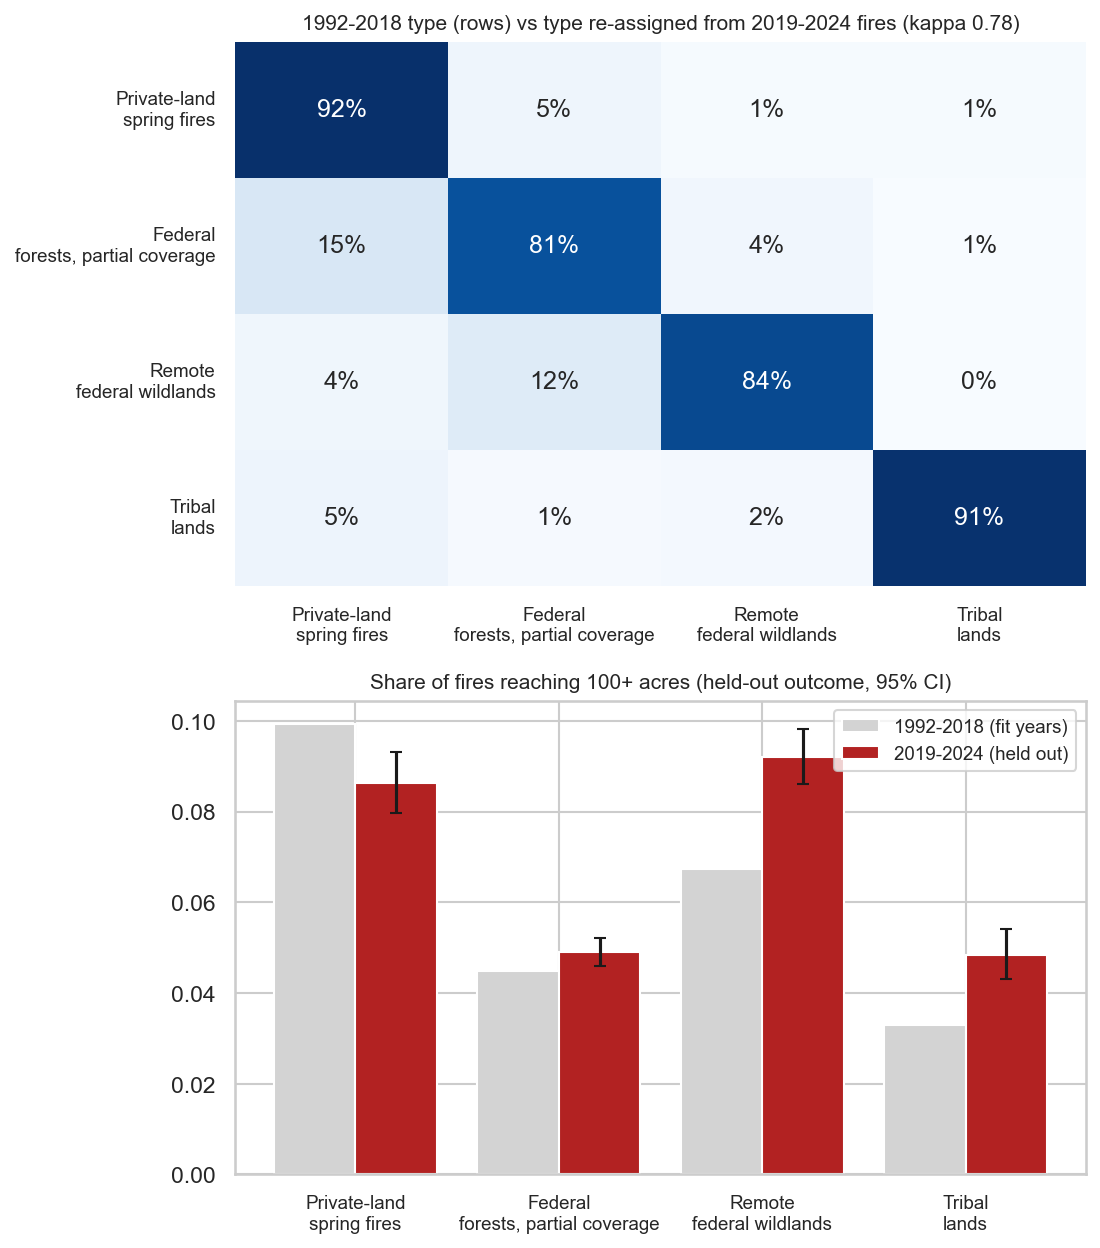
\includegraphics[width=\columnwidth]{temporal_validation.png}
\caption{Temporal check. Top: type in 1992--2018 (rows) vs the type assigned from 2019--2024 fires alone with the 1992--2018 scaler and centres (1{,}288 cells with 10+ recent fires). Bottom: share of fires reaching 100 acres by type, a held-out outcome, in the fit years and in 2019--2024 (95\% Wilson intervals).}
\label{fig:temporal}
\end{figure}

\subsection{What drives the partition}
Dropping station access (ARI 0.38) or land owner (0.41) changes the partition most, then season (0.62). Fire rate (0.87), discovery hour (0.87) and weekend share (0.97) matter little. This differs from the Milestone~1 preliminary clustering, where distance mattered little because fire-size features dominated it. With size moved to the held-out side, how far help is becomes a main axis of the typology.

\subsection{Association rules}
2{,}916 candidate rules meet the support threshold ($z=4.14$ after Bonferroni), and \textbf{121} pass the lift and non-redundancy filters. On 2019--2024, which they never saw, 98\% keep lift above 1 and 88\% keep lift $\geq 2$; the Spearman correlation of the two lifts is 0.66 (Figure~\ref{fig:rules}). The strongest rules (Table~\ref{tab:rules}) combine \emph{distance}, \emph{private land} and \emph{remote cells}. Fires 20+~km from any station on Plains land in sparse cells become large 28\% of the time, against 2.9\% overall.

\begin{figure}[!htb]
\centering
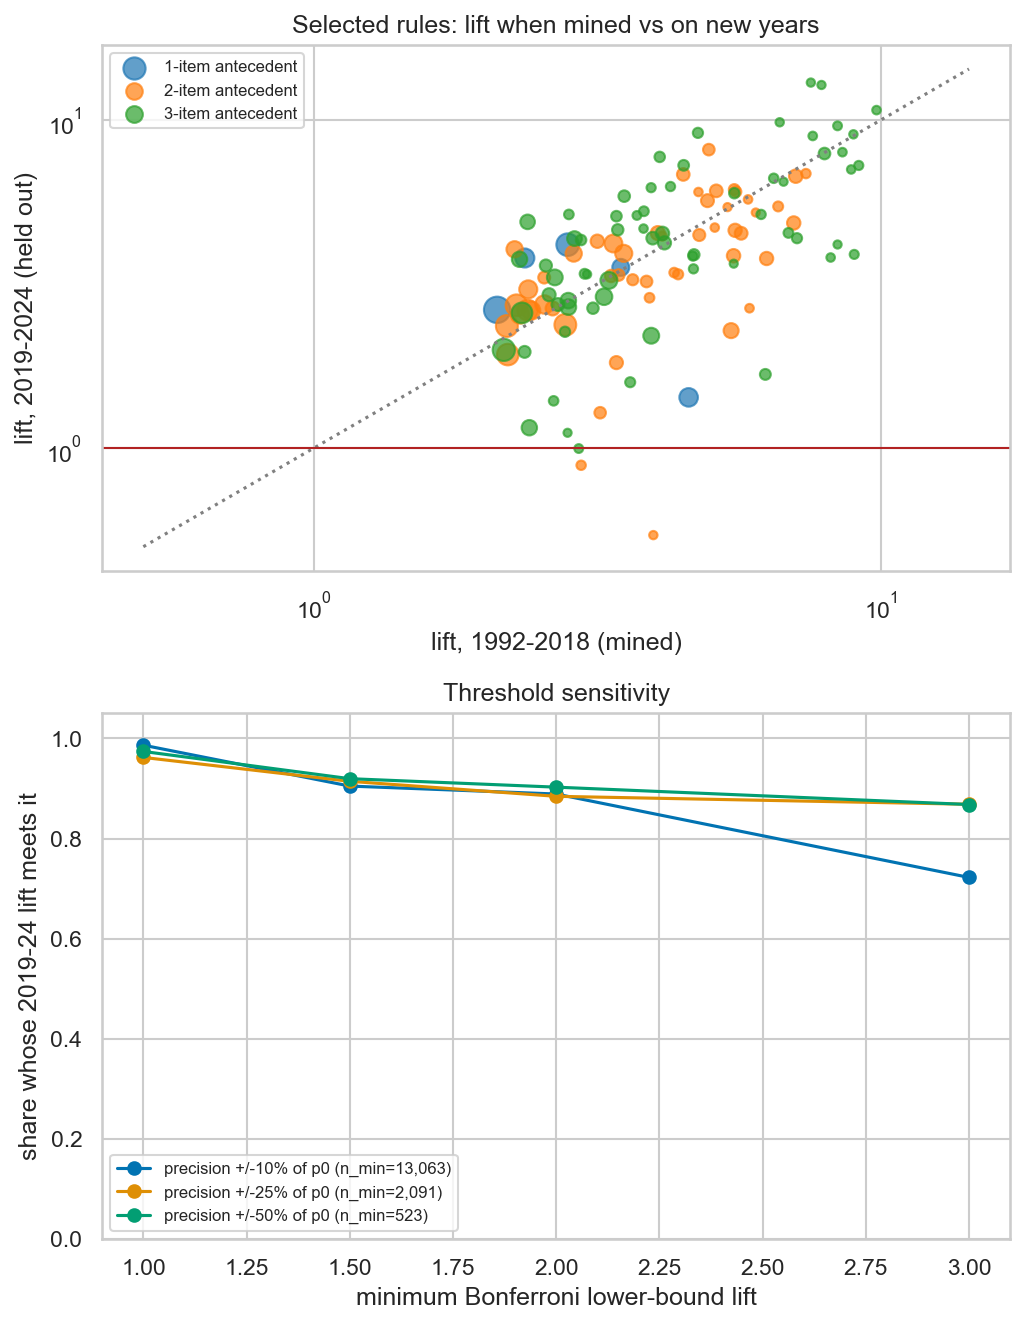
\includegraphics[width=\columnwidth]{association_rules.png}
\caption{Association rules. Top: lift of the 121 selected rules on the mining years (1992--2018) and on the held-out 2019--2024 fires; point size $\propto\sqrt{\text{matches}}$, dotted line = equal lift, red line = lift 1. Bottom: share of rules whose 2019--2024 lift still meets the threshold, for three support levels and four lift thresholds.}
\label{fig:rules}
\end{figure}

The rules also tie back to the types. Private-land spring fires appear in 10 rules, tribal lands in none. Within both federal types, the risky fires are on \emph{private in-holdings}: lift 2.4 in federal forests and 3.8 in remote wildlands (Mountain West), rising to 4.7 in 2019--2024. Of the 14 rules that fall below lift 2 in 2019--2024, six rest on administrative items (missing cause, missing or state/local owner, unknown time), whose coding changed in 2020--21.

\begin{table}[!htb]
\centering\footnotesize
\setlength{\tabcolsep}{2.5pt}
\caption{Top selected rules (consequent: fire reaches 100+ acres) by Bonferroni lower-bound lift $\ell/p_0$, plus the best rule for two types. $n$ = matching 1992--2018 fires.}
\label{tab:rules}
\begin{tabularx}{\columnwidth}{@{}Xrcccc@{}}
\toprule
Antecedent & $n$ & Conf. & Lift & $\ell/p_0$ & Lift'19 \\
\midrule
Plains, 20+ km, sparse cell & 2{,}649 & 28.1\% & 9.83 & 8.62 & 10.72 \\
private, 20+ km, sparse cell & 3{,}452 & 26.1\% & 9.15 & 8.11 & 7.27 \\
private, Natural, sparse cell & 3{,}290 & 25.7\% & 8.98 & 7.92 & 3.89 \\
Plains, day, \emph{private spring} type & 2{,}421 & 25.6\% & 8.95 & 7.73 & 9.05 \\
Plains, Natural, sparse cell & 2{,}577 & 25.3\% & 8.87 & 7.69 & 7.07 \\
Plains, private, 20+ km & 2{,}995 & 24.0\% & 8.39 & 7.31 & 9.60 \\
\midrule
Mtn West, private, \emph{remote federal} & 2{,}569 & 10.9\% & 3.82 & 3.01 & 4.67 \\
private, day, \emph{federal partial} & 9{,}742 & 6.7\% & 2.35 & 2.01 & 1.96 \\
\bottomrule
\end{tabularx}
\end{table}

\paragraph{Threshold sensitivity.} The thresholds are not fragile (Figure~\ref{fig:rules}, bottom). Across precision targets of $\pm$50\%, $\pm$25\% and $\pm$10\% ($n_{\min}$ = 523, 2{,}091, 13{,}063) and lift thresholds of 1--3, 96--100\% of selected rules keep lift above 1 on new years. 87--92\% keep their lift threshold, except at the strictest corner ($\pm$10\%, lift $\geq$3: 72\% of 18 rules). Loosening to $\pm$50\% adds 33 rules at the same replication rate; tightening to $\pm$10\% leaves 45. The chosen setting is the middle of this range.

%=====================================================================
\section{Discussion and Limitations}
%=====================================================================
\paragraph{Answer to RQ2 (preliminary).} Under-served wildfire country is not one problem. It falls into four reproducible types, and each points to a different kind of help (Table~\ref{tab:help}). Only one of them, private-land spring fires, is a natural candidate for new structural stations. This matches the Milestone~1 coverage experiment: 200 extra stations raised coverage of recent large fires by only 4 points.

\begin{table}[!htb]
\centering\footnotesize
\caption{From types to operational help.}
\label{tab:help}
\begin{tabularx}{\columnwidth}{@{}lX@{}}
\toprule
Type & What help fits \\
\midrule
Remote federal wildlands & Detection, aviation, pre-positioned federal initial attack; large-fire rate rising (9.2\% in 2019--24) \\
Federal forests, partial & Federal crews already contain most fires (4.9\% large); focus on private in-holdings and complexes \\
Private-land spring fires & Rural and volunteer stations, burn restrictions and prevention in the Plains (8.6--9.9\% large) \\
Tribal lands & Tribal and BIA fire programmes; low large-fire rate, many small fires \\
\bottomrule
\end{tabularx}
\end{table}

\begin{itemize}
\item \textbf{Sparse cells are left out.} Cells with fewer than 30 fires cannot be described reliably, yet they hold 26 of the 100 largest fires. They need a separate fire-level treatment.
\item \textbf{Overlapping types.} Silhouettes of 0.09--0.27 mean the borders are fuzzy; border cells should be read with care.
\item \textbf{Administrative signal.} Owner and discovery-time fields are partly reporting artefacts, so the types reflect \emph{how} fires are reported as well as how they behave. We report this as a finding but it limits a purely physical reading.
\item \textbf{Station data.} The layer is a recent snapshot of mostly structural stations; federal wildland crews are missing, which overstates the gap on federal land (Milestones~1--2).
\item \textbf{Fixed grid.} The 25~km grid, 30-fire minimum and 10~km cut-off come from Milestone~1 and have not yet been varied.
\end{itemize}

%=====================================================================
\section{Next Steps (Optimisation Phase)}
%=====================================================================
\begin{enumerate}
\item Repeat the stability-based selection for 15, 25 and 40~km grids and 5--15~km under-served cut-offs, and report how the typology changes.
\item Give border cells soft memberships (fuzzy $c$-means, or Gaussian mixtures on de-duplicated owner features).
\item Build a separate, fire-level typology for sparse cells, where the largest fires are.
\item Feed the cell type and the top rules into the RQ1 model as engineered features and measure the PR-AUC gain.
\end{enumerate}

\paragraph{Reproducibility.} Data loading and the station join are in \code{src/features.py}; grid cells, cell features, stability, effect sizes and rule mining are in \code{src/clustering.py}, with unit tests in \code{tests/test_clustering.py}. Pinned versions are in \code{requirements.txt}. Paths are found relative to the repository and all seeds are fixed (281). The notebook reuses the Milestone~2 cache and runs in about 4 minutes.

\begin{thebibliography}{99}
\bibitem{short2026} K.~C. Short. \emph{Spatial wildfire occurrence data for the United States, 1992--2024 [FPA\_FOD\_20260615]}, 7th ed. USDA Forest Service Research Data Archive, Fort Collins, CO.
\bibitem{hifld} U.S. Geological Survey / DHS Homeland Infrastructure Foundation-Level Data (HIFLD). \emph{Fire and Emergency Medical Service (EMS) Stations}. Archived on DataLumos, project 239161. \url{https://www.datalumos.org/datalumos/project/239161}
\bibitem{benhur2002} A.~Ben-Hur, A.~Elisseeff and I.~Guyon. A stability based method for discovering structure in clustered data. In \emph{Pacific Symposium on Biocomputing}, 2002.
\bibitem{tibshirani2001} R.~Tibshirani, G.~Walther and T.~Hastie. Estimating the number of clusters in a data set via the gap statistic. \emph{Journal of the Royal Statistical Society B}, 63(2):411--423, 2001.
\bibitem{campello2013} R.~J.~G.~B. Campello, D.~Moulavi and J.~Sander. Density-based clustering based on hierarchical density estimates. In \emph{Proceedings of PAKDD}, 2013.
\bibitem{agrawal1994} R.~Agrawal and R.~Srikant. Fast algorithms for mining association rules. In \emph{Proceedings of VLDB}, 1994.
\bibitem{bayardo2000} R.~J. Bayardo, R.~Agrawal and D.~Gunopulos. Constraint-based rule mining in large, dense databases. \emph{Data Mining and Knowledge Discovery}, 4:217--240, 2000.
\end{thebibliography}

\end{document}
